\documentclass{scrartcl}

\usepackage{amssymb}
\usepackage{amsmath}
\usepackage{tikz}

%Mohssen, M., Khan, M., Bashier, E. (2016). \textit{Machine Learning: Algorithms and Applications}. Boca Raton, FL: CRC Press, ch. 6: "Neural Networks"

%Krenker, A., Bešter, J., Kos, A. (2011). ``Introduction to the Artificial Neural Networks,'' in Suzuki, K. (Ed.). (2011). \textit{Artificial Neural Networks: Methodological Advances and Biomedical Applications}. London: InTechOpen, ch. 1 (p. 5, fig. 3)

\begin{document}
	
	%\begin{figure}
	%	\centering
	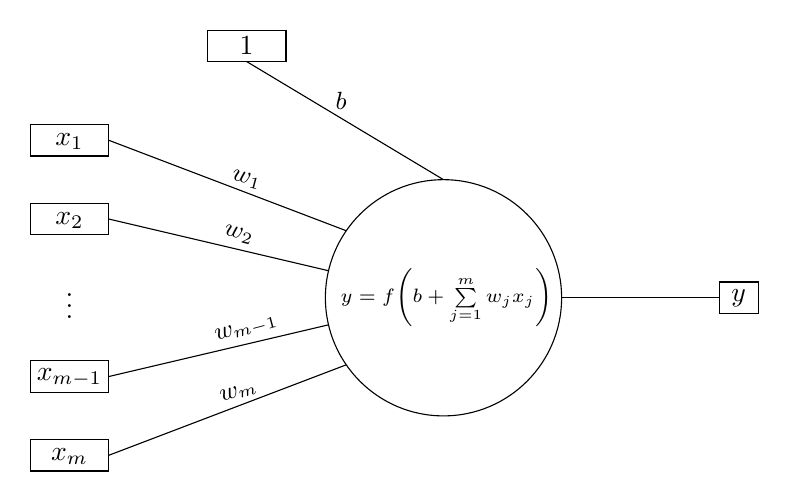
\begin{tikzpicture}
	%inputs (x)
	\draw (-5.25,1.8) rectangle (-4.25,2.2);	\node at (-4.75,1.98) {$x_1$};
	\draw (-5.25,0.8) rectangle (-4.25,1.2);	\node at (-4.75,0.98) {$x_2$};
	\node at (-4.75,0) {$\vdots$};
	\draw (-5.25,-0.8) rectangle (-4.25,-1.2);	\node at (-4.75,-1.02) {$x_{m-1}$};
	\draw (-5.25,-1.8) rectangle (-4.25,-2.2);	\node at (-4.75,-2.02) {$x_m$};
	
	%weights (w)
	\draw (-4.25,2)--(1,0);		\node at (-2.5,1.5) {\rotatebox{-15}{\small $w_1$}};
	\draw (-4.25,1)--(0,0);		\node at (-2.6,0.8) {\rotatebox{-15}{\small $w_2$}};
	\draw (-4.25,-1)--(0,0);	\node at (-2.5,-.4) {\rotatebox{15}{\small $w_{m-1}$}};
	\draw (-4.25,-2)--(1,0);	\node at (-2.6,-1.2) {\rotatebox{15}{\small $w_m$}};
	
	%bias (b)
	\draw (-3,3) rectangle (-2,3.4);	\node at (-2.5,3.2) {$1$};
	\draw (-2.5,3)--(0,1.5);			\node at (-1.3,2.5) {\small $b$};
	
	%output (y) on right
	\draw (1.5,0)--(3.5,0);
	\draw (3.5,-0.2) rectangle (4,0.2);		\node at (3.75,0) {$y$};
	
	\filldraw[fill=white] (0,0) circle (1.5);
	\node at (0,0) {{\scriptsize $\;y = f\!\left(b+ \sum\limits_{j=1}^m w_jx_j\right)$}};
	%\draw[help lines] (-6,-2) grid (4,4);
	\end{tikzpicture}
	%	\caption{A perceptron with $m$ inputs and a bias (Mohssen, Khan, \& Bashier, 2016: 93)}
	%\end{figure}
	
	\vspace{2cm}
	
	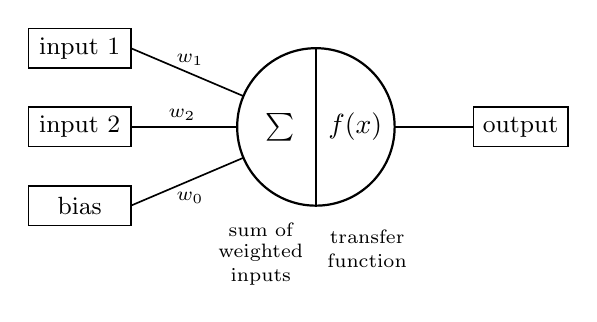
\begin{tikzpicture}
	%inputs
	\draw[semithick] (-3.65,0.75) rectangle (-2.35,1.25);
	\node at (-3,1) {\small input 1};
	\draw[semithick] (-2.35,1)--(0,0);
	\node at (-1.6,0.85) {\scriptsize $w_1$};
	%
	\draw[semithick] (-3.65,-0.25) rectangle (-2.35,0.25);
	\node at (-3,0) {\small input 2};
	\draw[semithick] (-2.35,0)--(0,0);
	\node at (-1.7,0.15) {\scriptsize $w_2$};
	%
	\draw[semithick] (-3.65,-0.75) rectangle (-2.35,-1.25);
	\node at (-3,-1) {\small bias};
	\draw[semithick] (-2.35,-1)--(0,0);
	\node at (-1.6,-0.9) {\scriptsize $w_0$};
	
	%circle
	\filldraw[fill=white,thick] (0,0) circle (1);
	\draw[thick] (0,1)--(0,-1);
	\node at (-0.45,0) {$\sum$};
	\node at (0.5,0) {$f(x)$};
	
	%output
	\draw[semithick] (1,0)--(2,0);
	\draw[semithick] (2,-0.25) rectangle (3.2,0.25);
	\node at (2.6,0) {\small output};
	
	%labels
	\node at (-.7,-1.3) {\scriptsize sum of};
	\node at (-.7,-1.6) {\scriptsize weighted};
	\node at (-.7,-1.9) {\scriptsize inputs};
	%
	\node at (0.65,-1.4) {\scriptsize transfer};
	\node at (0.65,-1.7) {\scriptsize function};
	\end{tikzpicture}
	
\end{document}